\section{Reconstruction des événements}\label{chapter-LHC-section-evt_reco}
L'analyse des événements à partir des signaux bruts issus du détecteur n'est pas aisée, qu'il s'agisse de données réelles ou simulées.
Une interprétation de ces signaux en termes de particules physiques donne un point de départ beaucoup plus accessible.
%En effet, ces signaux sont comme des \og symptômes \fg{} du passage des particules dans le détecteur.
%La reconstruction des événements consiste donc en un \og diagnostic \fg{} de l'événement.
Pour y parvenir, un algorithme de reconstruction est utilisé.
Son rôle est de déterminer quelles particules sont issues de la collision étant donnés les signaux dans le détecteur.
Cette reconstruction est réalisée de manière identique dans les données réelles et simulées.
\par
Les signaux caractéristiques des différents types de particules dans le plan transverse du détecteur CMS sont illustrés sur la figure~\ref{fig-chapter-LHC-section-evt_reco-cms_slice}.
Il s'agit de la conséquence directe de la description du détecteur de la section~\ref{chapter-LHC-section-CMS}.
La plupart des particules laissent des signaux dans plusieurs sous-détecteurs.
Pour une particule donnée, ces signaux doivent donc présenter une corrélation.
\begin{figure}[b]
\includegraphics[width=\textwidth]{\PhDthesisdir/plots_and_images/CMS_slices/own/all_ptcs.tex}
\caption[Coupe transverse schématique du détecteur CMS.]{Coupe transverse schématique du détecteur CMS et signaux caractéristiques laissés par les particules. Les hadrons forment un dépôt dans le HCAL. Les hadrons chargés présentent de plus une trace dans le trajectographe dont l'extrapolation doit passer par ce dépôt. De même, les photons et électrons forment un dépôt dans le ECAL et les électrons présentent une trace dans le trajectographe dont l'extrapolation doit passer par ce dépôt. Enfin, les muons se propagent à travers tout le détecteur et laissent une trace dans les chambres à muons dont l'extrapolation doit correspondre à une trace du trajectographe. Dans toute la suite de ce manuscrit, les schémas des événements dans le détecteur utilisent la même présentation, en particulier pour les couleurs des sous-détecteurs et des particules. Réalisé à l'aide de CMSTransverseTikZ~\cite{CMSTransverseTikZ}.}
\label{fig-chapter-LHC-section-evt_reco-cms_slice}
\end{figure}
\par La reconstruction des événements se fait ainsi en combinant les informations issues des différents sous-détecteurs.
Un algorithme spécialement développé afin d'optimiser cette combinaison, l'algorithme de reconstruction du flux de particules (\PF, \emph{Particle Flow})~\cite{particle-flow,Dordevic_particle_flow}, a pour rôle de réaliser cette reconstruction.
Dans un premier temps, l'algorithme de \PF\ reconstruit les éléments d'identification des particules à partir des signaux de chaque sous-détecteur.
Dans un second temps, ces éléments d'identification sont combinés afin de reconstruire les particules de l'événement.
Des objets physiques plus complexes, dits de \og haut niveau \fg, sont également définis à partir de ces particules individuelles.
Il s'agit des jets, de l'énergie transverse manquante et des taus hadroniques.
\subsection{Éléments d'identification du \emph{Particle Flow}}\label{chapter-LHC-section-evt_reco-subsec-PF_elements}
\subsubsection{Traces des particules chargées et vertex}\label{chapter-LHC-section-evt_reco-subsec-PF_elements-subsubsec-tracks}
\paragraph{Traces des particules chargées}
Les particules chargées laissent des traces de leur passage dans le trajectographe et, dans le cas des muons, dans les chambres à muons.
Le trajectographe, présenté section~\ref{chapter-LHC-section-CMS-subsec-tracker}, ne donne pas de traces continues mais des points de passage de ces particules.
\par
Les traces des particules sont reconstruites à partir de ces points de passage à l'aide d'une méthode itérative~\cite{particle-flow,track_reco}.
Un détecteur de traces par combinaison basé sur un filtre de Kalman (KF) \cite{Kalman_filter} reconstruit les traces selon la procédure suivante:
\begin{enumerate}
\item Une trajectoire initiale est générée à partir d'un ajustement à quelques points de passages.
Cette trajectoire doit être compatible avec celle d'une particule chargée.
\item L'ensemble des points de passage devant correspondre à cette trajectoire est déterminé.
Ces points sont obtenus en extrapolant la trajectoire à travers le trajectographe.
À chaque ajout d'un point de passage, l'ajustement de la trajectoire à l'ensemble des points lui étant associés est mis à jour.
\item Une fois que l'ensemble des points pouvant être associés à la trajectoire ont été trouvés, un ajustement final est réalisé.
Il permet de déterminer l'ajustement optimal de la trajectoire aux points de passage.
Les propriétés de la particule chargée (origine, impulsion transverse, direction) sont ainsi déterminées.
La trace est acceptée ou rejetée selon des critères portant sur les paramètres de l'ajustement final.
Les points de passage associés à une trace acceptée sont retirés de la liste des points à traiter.
\end{enumerate}
Cette procédure est alors répétée en utilisant des critères de plus en plus précis afin d'augmenter l'efficacité de la reconstruction des traces.
Le taux de mauvaise reconstruction est quant à lui réduit en appliquant des critères de qualité sur les traces reconstruites.
%Plus de détails sont disponibles dans la référence~\cite{particle-flow}.
\subparagraph{Cas des électrons}
La reconstruction des électrons de haute énergie et isolés vis-à-vis des autres particules est naturellement basée sur les données du ECAL~\cite{electron_reco_8tev}.
La position et la valeur du dépôt d'énergie sont utilisés afin de déterminer les points de passage attendus dans le trajectographe pour l'électron (ou le positron).
Cependant, à cause de l'épaisseur du trajectographe, les électrons émettent avant de parvenir au ECAL une fraction de leur énergie par \emph{bremsstrahlung}, \ie\ sous forme de photons.
Les performances de reconstruction des électrons dépendent ainsi fortement de la capacité à identifier ces photons et mesurer leurs énergies.
Les dépôts d'énergie dans le ECAL (\emph{clusters}) dus à l'électron et aux photons potentiellement issus du \emph{bremsstrahlung} sont regroupés en un \emph{supercluster}.
Le \emph{supercluster} est construit à partir des dépôts du ECAL se situant dans une fenêtre fine en $\eta$ et plus large en $\phi$ afin de prendre en compte la courbure de la trajectoire de l'électron due au champ magnétique.
\par
Dans le cas des électrons contenus dans les jets, en revanche, un biais apparaît à cause des autres particules du jet situées à proximité de l'électron.
Cet effet mène à un fort taux de mauvaise reconstruction.
L'identification des électrons à partir du ECAL est ainsi limitée aux cas d'électrons isolés des autres particules.
Afin de reconstruire les électrons exclus par cette limitation, une approche basée sur les données du trajectographe a été développée~\cite{particle-flow}.
Dès qu'une trace reconstruite selon la procédure exposée précédemment vérifie $\pT>\SI{2}{\GeV}$, elle est considérée comme candidat électron.
\par
Lorsque l'électron émet peu d'énergie par \emph{bremsstrahlung}, l'ajustement de la trace correspondante est de bonne qualité à travers l'ensemble du trajectographe.
De plus, l'extrapolation de cette trace jusqu'à la surface du ECAL permet de lui faire correspondre un dépôt d'énergie.
L'énergie contenue dans le dépôt doit alors être compatible avec celle déterminée à partir de la trace.
\par
Plus l'électron émet de l'énergie par \emph{bremsstrahlung}, moins l'ajustement de la trace correspondante est de qualité, car cet ajustement ne prend pas en compte la perte d'énergie au cours de la propagation de l'électron.
Les traces correspondant à cette situation sont sélectionnées à partir du nombre de points de passage associés et du $\chi^2$ de l'ajustement.
Elles sont réajustées à partir d'un filtre de somme de gaussiennes (GSF, \emph{Gaussian Sum Filter}) \cite{GSF} utilisant cinq paramètres, plus adapté que le KF pour ces électrons~\cite{particle-flow}.
Un critère d'identification basé sur un arbre de décision (BDT, \emph{Bossted Decision Tree}) est appliqué sur cet ajustement, il est détaillé dans la section~\ref{chapter-LHC-section-evt_reco-subsec-ptc_ID}.
\subparagraph{Cas des muons}
%Les chambres à muons permettent d'identifier ces particules avec une grande efficacité.
%Les calorimètres, situés entre le point de collision et les chambres à muons, absorbent toutes les autres particules (à l'exception des neutrinos qui n'interagissent pas), permettant d'obtenir une bonne pureté quant aux particules se propageant dans les chambres à muons.
Les muons laissent des signaux de leur passage dans le trajectographe et dans les chambres à muons.
Trois types de muons peuvent être définis:
\begin{itemize}
\item les muons seuls (\emph{standalone muons}), reconstruits uniquement à partir des signaux des chambres à muons;
\item les muons globaux (\emph{global muons}), obtenus par la correspondance d'une trace dans le trajectographe avec l'extrapolation de la trace d'un muon seul;
\item les muons du trajectographe (\emph{tracker muons}) sont les traces du trajectographe d'impulsion transverse supérieure à \SI{0.5}{\GeV} dont l'extrapolation passe par une des chambres à muons ayant détecté le passage d'une particule.
\end{itemize}
\par
Lorsque des hadrons chargés arrivent au HCAL, ils se désintègrent en une gerbe hadronique.
Si des éléments de cette gerbe parviennent à traverser le HCAL (\emph{punch-through}), ils donnent un signal dans les chambres à muons.
Des critères d'identification sont alors appliqués aux traces afin de réduire les muons reconstruits à partir de hadrons.
Ils sont abordés dans la section~\ref{chapter-LHC-section-evt_reco-subsec-ptc_ID}.
\paragraph{Interactions avec le matériau du trajectographe}
Des interactions entre les particules issues des collisions et le matériau du trajectographe peuvent mener
à une déviation (\emph{kink})~\cite{moliere_scat_1,moliere_scat_2}
voire
à la production de vertex secondaires~\cite{particle-flow,CMS-TRK-17-001},
comme illustré sur la figure~\ref{fig-chapter-LHC-section-evt_reco-subsec-PF_elements-CMS-self-radio}.
Un algorithme a été développé~\cite{CMS-PAS-TRK-10-003} afin d'identifier les traces de particules ayant interagit avec le matériau du trajectographe.
\begin{figure}[h]
\centering
\subcaptionbox{Dans le plan longitudinal \plane{r}{z}.\label{subfig-chapter-LHC-section-evt_reco-subsec-PF_elements-particle-flow-Figure_005-a}}[.45\textwidth]
{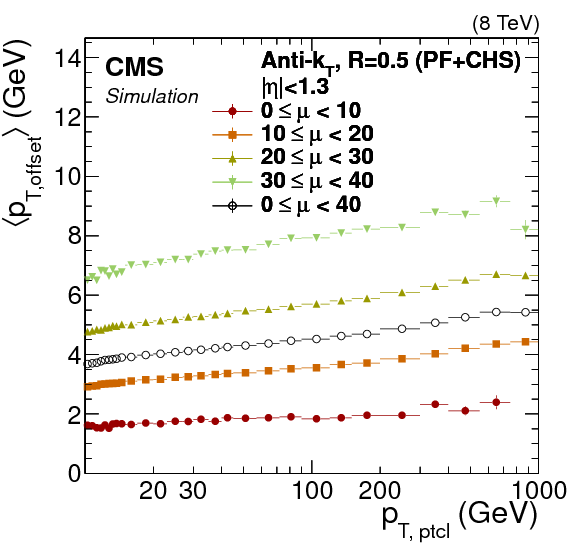
\includegraphics[width=.45\textwidth]{\PhDthesisdir/plots_and_images/from_particle-flow/Figure_005-a.png}}
\hfill
\subcaptionbox{Dans le plan transverse \plane{x}{y}.\label{subfig-chapter-LHC-section-evt_reco-subsec-PF_elements-particle-flow-Figure_005-b}}[.45\textwidth]
{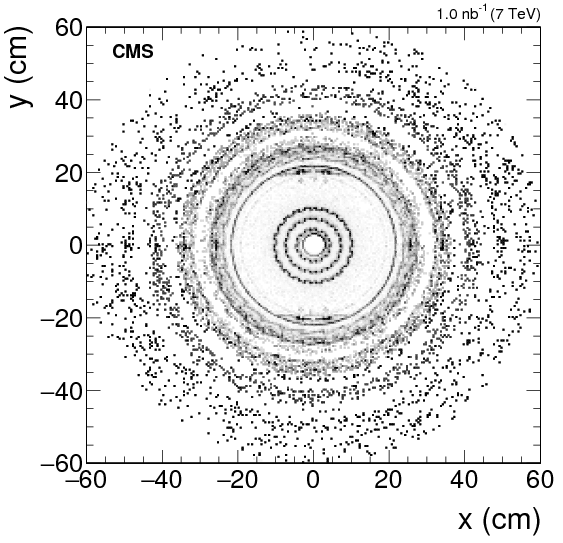
\includegraphics[width=.45\textwidth]{\PhDthesisdir/plots_and_images/from_particle-flow/Figure_005-b.png}}
\caption[Points d'interactions entre particules des événements et matière composant le détecteur.]{Carte des points d'interactions entre particules des événements et matière composant le détecteur~\cite{particle-flow,CMS-TRK-17-001} à partir de données prises en 2011 à $\sqrt{s}=\SI{7}{\TeV}$.}
\label{fig-chapter-LHC-section-evt_reco-subsec-PF_elements-CMS-self-radio}
\end{figure}
\paragraph{Vertex}
La combinaison des traces permet de reconstruire les vertex d'interactions de l'événement.
Plusieurs vertex sont présents du fait de l'empilement.
Le vertex principal est choisi comme étant le vertex dont la somme des impulsions transverses au carré des traces en provenant est la plus élevée, les autres sont considérés comme des vertex de l'empilement.
L'efficacité de reconstruction du vertex principal est ainsi de l'ordre de \SI{100}{\%}, celle des vertex de l'empilement de \SI{70}{\%}~\cite{JERC_RunI}.
\subsubsection{Dépôts dans les calorimètres}
\paragraph{Agglomération}
Les dépôts dans les calorimètres sont regroupés de proche en proche en agglomérats (\emph{clusters})~\cite{particle-flow}, indépendamment pour chaque sous-partie des calorimètres.
Plusieurs raisons existent à cette agglomération:
\begin{itemize}
\item détecter et mesurer les énergies et directions des particules neutres stables comme les photons et les hadrons neutres;
\item séparer ces particules neutres des particules chargées;
\item reconstruire et identifier les électrons et les photons issus du \emph{bremsstrahlung} correspondant;
\item améliorer la mesure de l'énergie des hadrons chargés dont les traces sont imprécises.
\end{itemize}
\par La construction de ces agglomérats commence par l'identification des cellules des calorimètres mesurant une énergie supérieure à un seuil, défini pour chaque sous-partie des calorimètres.
Les seuils sont fixés à partir d'une optimisation sur des simulations de photons, \pionnull, \Kaonnull\ et jets.
Les cellules adjacentes sont ajoutées à l'agglomérat.
Puis, toute cellule avec au moins un coin en commun avec une cellule déjà dans l'agglomérat et mesurant une énergie supérieure à deux fois le niveau moyen du bruit est ajoutée à l'agglomérat.
%\par
%Afin d'identifier les photons issus du \emph{bremsstrahlung} d'un électron, les dépôts dans le ECAL pouvant correspondre à l'électron et à ces éventuels photons sont regroupés en un \emph{supercluster}.
%Le \emph{supercluster} est ainsi l'ensemble des \emph{clusters} dans le ECAL se situant à proximité de la direction de l'électron~\cite{particle-flow}.
\paragraph{Calibration}
Les photons et les hadrons neutres sont reconstruits à l'aide de leurs dépôts dans les calorimètres.
Des dépôts isolés vis-à-vis des traces de particules chargées sont une signature claire des particules neutres.
Cependant, un dépôt de particule neutre situé au même endroit qu'un dépôt de particule chargée ne peut être détecté que comme étant un excès d'énergie pour la particule chargée par rapport à l'énergie déterminée à l'aide du trajectographe.
Une bonne calibration de la réponse des calorimètres aux photons et aux hadrons est donc cruciale pour la bonne reconstruction des particules neutres.
Cette calibration a été réalisé dans un premier temps avant les premières collisions à l'aide de faisceaux de test.
Une fois les collisions commencées, les données issues des celles-ci sont exploitées afin de calibrer plus finement les calorimètres.
%Plus de détails sont disponibles dans la section~3.5 de la référence~\cite{particle-flow}.
\subsection{Identification et reconstruction des particules}\label{chapter-LHC-section-evt_reco-subsec-ptc_ID}
Des éléments d'identification du \PF\ dans différents sous-détecteurs sont généralement dus à une même particule.
La reconstruction des particules se fait alors par association de ces éléments.
L'association des éléments dus à une particule est uniquement limitée par la granularité des sous-détecteurs et par le nombre de particules par unité d'angle solide~\cite{particle-flow}.
De même, l'association de tous les éléments dus à une seule particule est limitée par la quantité de matière traversée en amont des calorimètres ou, le cas échéant, des chambres à muons, pouvant dévier la particule~\cite{moliere_scat_1,moliere_scat_2}.
\par Un algorithme teste les paires d'éléments de reconstruction possibles.
Afin de limiter les temps de calcul, seules les paires d'éléments les plus proches entre eux dans le plan $(\eta,\phi)$ sont considérées.
Des conditions supplémentaires sont requises afin d'associer deux éléments et sont détaillées dans les sections suivantes.
Lorsque deux éléments sont associés, une distance est définie par l'algorithme afin de quantifier la qualité de cette association.
Des \og blocs \fg{} du \PF\ sont ainsi obtenus par association des éléments de reconstruction.
Selon le contenu de ce bloc, un type de  particule est reconstruit.
Ces différents types de particules sont détaillés dans les sections qui suivent.
\subsubsection{Muons}
Les muons sont reconstruits à partir des éléments d'identifications que sont les muons globaux, seuls et du trajectographe définis dans la section~\ref{chapter-LHC-section-evt_reco-subsec-PF_elements-subsubsec-tracks}.
\par Tout d'abord, les muons globaux isolés, \ie\ sans autre activité dans le voisinage de la trajectoire correspondante, sont sélectionnés~\cite{particle-flow}.
Les traces additionnelles et les dépôts d'énergie dans les calorimètres se situant dans un cône de rayon $\Delta R$ inférieur à \num{0.3} dans le plan $(\eta,\phi)$, où
\begin{equation}
\Delta R_{ij}^2 = (\eta_i-\eta_j)^2 + (\phi_i-\phi_j)^2
\mend[,]
\end{equation}
sont également associés au muon global.
Il est requis que la somme des impulsions transverses et des énergies de ces traces et dépôts n'excède pas \SI{10}{\%} de l'impulsion transverse du muon global.
Ce critère est suffisant pour rejeter les hadrons réussissant à traverser le HCAL.
Ensuite, les muons globaux non isolés sont sélectionnés à l'aide d'un critère d'identification strict (\emph{Tight muon ID})~\cite{CMS-MUO-16-001} auquel la présence d'au moins trois segments de trace compatibles est requise.
\par Les muons non identifiés à ce stade peuvent l'être en utilisant les muons seuls et les muons du trajectographe.
Les muons seuls présentant un grand nombre de signaux dans les chambres à muons, au moins 23 dans les DT (pour un maximum possible de 32) ou 15 dans les CSC (pour un maximum possible de 24), et dont l'ajustement de la trace à ces signaux est de bonne qualité sont ainsi retenus.
Les muons du trajectographe sont également retenus s'ils contiennent au moins 13 points de passage dans le trajectographe et que les agglomérats dans les calorimètres sont compatibles avec la traduction de la trace correspondante en tant que muon.
\par Jusqu'à $\pT=\SI{100}{\GeV}$, la résolution en énergie des muons reconstruits par cette méthode est de \SI{1}{\%} dans le barillet et de \SI{3}{\%} dans les bouchons~\cite{CMS-MUO-16-001}.
L'efficacité de reconstruction est de \SI{95}{\%} et le taux d'identification de hadrons en tant que muons inférieur à \SI{1}{\%}.
Les éléments d'identification du \PF\ utilisés pour reconstruire les muons sont retirés dans la suite du processus de reconstruction de l'événement.
\subsubsection{Électrons et photons isolés}
L'identification des électrons et des photons isolés se base sur les éléments d'identification du \PF\ provenant du trajectographe et du ECAL.
De par la présence de la matière du trajectographe, les électrons émettent des photons par \emph{bremsstrahlung} et les photons se convertissent en paires $\antielectron\electron$, ces électrons étant également sujets au \emph{bremsstrahlung}, etc.
C'est pour cela qu'électrons et photons isolés sont traités de manières similaires pour leur reconstruction.
\par Un candidat électron est défini lorsqu'une trace du trajectographe, extrapolée jusqu'au ECAL, est associée à un dépôt d'énergie, si ce dépôt n'est pas lui-même relié à trois autres traces ou plus.
Les candidats photons isolés correspondent aux dépôts du ECAL avec une énergie transverse supérieure à \SI{10}{\GeV} n'étant pas associé à une trace.
Pour tous ces candidats, la somme des énergies mesurées dans les cellules du HCAL se situant dans un cône de rayon $\Delta R$ inférieur à \num{0.15} dans le plan $(\eta,\phi)$ ne doit pas correspondre à plus de \SI{10}{\%} de l'énergie du dépôt du ECAL.
Les traces identifiées comme celles de conversions de photons et les dépôts du ECAL associés sont de plus rattachées au candidat initial.
\par Les électrons et photons isolés sont alors obtenus en soumettant aux candidats définis précédemment des critères d'identification, prenant en compte jusqu'à 14 variables~\cite{particle-flow}.
Les définitions exactes de ces critères varient d'une année à l'autre en fonction des performances du détecteur et plusieurs niveaux d'exigence existent.
Les éléments d'identification du \PF\ utilisés pour reconstruire les électrons et photons isolés sont retirés dans la suite du processus de reconstruction de l'événement.
\subsubsection{Hadrons et photons non isolés}
Les muons, électrons et photons isolés ayant été reconstruits, seuls les hadrons et les photons non isolés issus de la formation des jets et de l'hadronisation\footnote{La formation des jets ainsi que l'hadronisation sont détaillées dans la section~\ifref{chapter-JERC-section-jets}{\ref{chapter-JERC-section-jets-subsec-hadronisation}}{2} du chapitre~\ifref{chapter-JERC}{\ref{chapter-JERC}}{4}.} restent à être reconstruits.
Ces particules sont généralement détectées comme des hadrons chargés (\pionpm, \Kaonpm, protons), des hadrons neutres (\Kaonlong, neutrons), des photons non isolés (désintégrations des \pionnull) et plus rarement comme des muons (désintégrations de hadrons lourds\footnote{La phénoménologie de la désintégration des hadrons lourds est abordée dans la section~\ifref{chapter-JERC-section-jets}{\ref{chapter-JERC-section-jets-subsec-hadronisation}}{2} du chapitre~\ifref{chapter-JERC}{\ref{chapter-JERC}}{4}.}).
\par Dans la région d'acceptation du trajectographe ($\abs{\eta}<\num{2.5}$), les photons non isolés et les hadrons neutres sont reconstruits respectivement à partir des dépôts d'énergie dans les ECAL et HCAL non associés à une trace.
Une priorité est donnée aux photons dans la mesure où \SI{25}{\%} de l'énergie des jets est portée par ces particules alors que seulement \SI{3}{\%} de l'énergie des jets est déposée dans le ECAL par les hadrons neutres.
Au-delà de l'acceptation du trajectographe, il n'est pas possible de faire la distinction entre hadrons neutres et chargés.
Près de \SI{25}{\%} de l'énergie des jets est ainsi déposée dans le ECAL et les agglomérats du ECAL se situant dans la même région qu'un agglomérat du HCAL sont considérés comme dus à la même gerbe hadronique, \ie\ au même hadron.
Les autres dépôts du ECAL sont considérés comme dus à des photons.
\par Les hadrons chargés sont identifiés à partir des agglomérats restant dans le HCAL, associés aux traces dans le trajectographe non utilisées pour l'identification des particules précédentes.
Ces traces peuvent elles-mêmes être reliées à un agglomérat résiduel du ECAL.
Pour chaque bloc du \PF\ ainsi construit, l'énergie dans les calorimètres est comparée à la somme des moments des traces.
Si un excès est observé avec les calorimètres, il est interprété comme la présence d'une particule neutre supplémentaire.
Si cet excès est inférieur à l'énergie dans le ECAL et plus grand que \SI{500}{\MeV}, alors la particule neutre est considérée comme étant un photon d'énergie égale à cet excès.
Sinon, l'énergie dans le ECAL donne un photon et si la partie de l'excès dans le HCAL est supérieure à \SI{1}{\GeV}, un hadron neutre est également considéré.
Puis, à partir de l'énergie calorimétrique restante, chaque trace du bloc du \PF\ donne un hadron chargé.


\section{Reconstruction des jets}\label{chapter-JERC-section-jets_reco}
Les particules colorées ne peuvent donc pas être directement observées dans le détecteur.
Leur signature expérimentale est un flux collimé de particules stables composé de hadrons, de leptons et de photons.
La présence de hadrons s'explique directement par le processus de hadronisation décrit dans la section précédente.
Les leptons proviennent de la désintégration, par interaction faible, des hadrons de saveur lourde, ou plus précisément des quarks de deuxième et troisième génération composant ces hadrons lourds.
Les photons sont radiés par les particules électriquement chargées.
\par Un processus physique comme celui de la figure~\ref{subfig-fgraph-Z_q_q} produit seulement quelques particules, en l'occurrence deux, et non des ensembles de particules, comme sur la figure~\ref{fig-agglo_hadronique} qui pourrait correspondre à l'état effectivement observé pour le processus de la figure~\ref{subfig-fgraph-Z_q_q}.
Afin de pouvoir étudier le processus initial, il est nécessaire de définir une observable décrivant les particules colorées à l'origine de ces flux collimés de particules stables.
\par Cette observable est un \og jet \fg.
À partir des particules identifiées à l'aide de l'algorithme de \emph{Particle Flow} (\PF)\footnote{L'algorithme de \emph{Particle Flow} est décrit dans la section~\ifref{chapter-LHC-section-evt_reco-subsec-PF}{\ref{chapter-LHC-section-evt_reco-subsec-PF}}{4.1} du chapitre\ifref{chapter-LHC}{~\ref{chapter-LHC}}{ \og Dispositif expérimental \fg}.}, un algorithme de regroupement permet d'obtenir la liste des jets de l'événement.
Il existe plusieurs algorithmes de regroupement dont le principe est décrit dans la section suivante.
\subsection{Algorithmes de regroupement}\label{chapter-JERC-section-jets_reco-subsec-algo}
Il existe deux catégories d'algorithmes permettant de regrouper les particules en jets, les algorithmes de cônes et les algorithmes de recombinaison séquentielle.
Dans la section~\ref{chapter-JERC-section-jets}, nous avons vu que les radiations de partons sont plus importantes pour de basses énergies (limite infrarouge) ou pour un parton radié colinéaire au parton initial (limite colinéaire).
Afin de conserver des prédictions de QCD vérifiables sur des jets réels, les algorithmes de regroupement doivent être insensibles à l'ajout d'une particule de basse énergie ou au partage d'une particule en deux particules d'énergies inférieures. C'est ce que l'on appelle l'insensibilité IRC, pour \emph{InfraRed and Colinear}.
La plupart des algorithmes de cônes ne sont pas IRC-insensibles, alors que la plupart des algorithmes de recombinaison séquentielle le sont.
\subsubsection{Les algorithmes de cônes}
Les algorithmes de cônes regroupent toutes les particules ayant une direction $\vec{p}$ telle que la distance $\Delta R_{pa}$ à la direction de l'axe du cône $\vec{a}$ dans le plan $(\eta,\phi)$\footnote{Les coordonnées $\eta$ et $\phi$ sont définies dans la section~\ifref{chapter-LHC-section-evt_reco-subsec-PF}{\ref{chapter-LHC-section-CMS-subsec-overview_and_coordinates}}{2.1} du chapitre\ifref{chapter-LHC}{~\ref{chapter-LHC}}{ \og Dispositif expérimental \fg}.} est inférieure à une distance de coupure $R_c$, \ie\ si
\begin{equation}
\Delta R_{pa} ^2 = (\eta_p - \eta_a)^2 + (\phi_p - \phi_a)^2 < R_c^2
\mend
\end{equation}
Alors, la direction $\vec{a}$ du cône et redéfinie comme étant la direction moyenne de toutes les particules rassemblées dans ce cône. Ce processus est itéré jusqu'à la stabilisation des cônes.
Enfin, les cônes sont séparés en cas de superposition, une particule ne pouvant appartenir qu'à un seul jet.
\par L'algorithme \textsc{SISCone}~\cite{SISCone}, \emph{Seedless Infrared Safe Cone}, est un exemple d'algorithme de cônes IRC-insensible.
Dans un premier temps, tous les cônes stables possibles sont reconstruits.
Ces cônes sont alors fusionnés, les cônes ayant l'impulsion transverse la plus grande absorbant des cônes d'impulsion transverse moindre dont ils contiennent déjà une fraction.
Un exemple de reconstruction de jets à l'aide de l'algorithme \textsc{SISCone} est présenté sur la figure~\ref{fig-chapter-JERC-section-jets_reco-subsec-algo-examples}.
\subsubsection{Les algorithmes de recombinaison séquentielle}
Les algorithmes de recombinaison séquentielle commencent par considérer que chaque particule forme un jet d'une seule particule.
Puis, à l'aide d'une métrique donnée, la paire de jets les plus proches entre eux fusionne en un seul jet tant que la distance entre eux est en-deçà d'une valeur seuil. Les jets fusionnés donnent la liste des jets de l'événement. Il est également possible de fixer le nombre de jets à déterminer et non la valeur seuil de la distance entre les jets à fusionner.
\par Plusieurs métriques peuvent être définies, chacune correspondant à un algorithme de recombinaison séquentielle proposant des regroupement différents.
\begin{description}
%\item[Algorithme de Durham] La distance $d_{ij}$ entre deux jets $i$ et $j$ est
%\begin{equation}
%d_{ij} = 2 \, \min(E_i^2, E_j^2) \, \frac{1-\cos\theta_{ij}}{Q^2}
%\end{equation}
%où $E_x$ est l'énergie du jet $x$, $\theta_{ij}$ l'angle entre les directions des deux jets et $Q$ l'énergie dans le centre de masse de la collision.
%Cet algorithme a l'avantage de regrouper les particules très fidèlement vis-à-vis de la gerbe hadronique, mais les jets obtenus possèdent une géométrie spatiale irrégulière, comme cela se voit sur la figure~\ref{fig-chapter-JERC-section-jets_reco-subsec-algo-examples}.
\item[Algorithme \kT] La distance $d_{ij}$ entre deux jets $i$ et $j$ est
\begin{equation}
d_{ij} = \min({\pT}_i^2, {\pT}_j^2) \, \frac{\Delta R_{ij}^2}{R^2}
\msep
\Delta R_{ij}^2 = (\eta_i-\eta_j)^2 + (\phi_i-\phi_j)^2
\end{equation}
où ${\pT}_x$ est l'impulsion transverse du jet $x$ et $R$ un paramètre libre.
Cet algorithme a l'avantage de regrouper les particules très fidèlement vis-à-vis de la gerbe hadronique, mais les jets obtenus possèdent une géométrie spatiale irrégulière, comme cela se voit sur la figure~\ref{fig-chapter-JERC-section-jets_reco-subsec-algo-examples}.
\item[Algorithme de Cambridge/Aachen] La distance $d_{ij}$ entre deux jets $i$ et $j$ est
\begin{equation}
d_{ij} = \frac{\Delta R_{ij}^2}{R^2}
\msep
\Delta R_{ij}^2 = (\eta_i-\eta_j)^2 + (\phi_i-\phi_j)^2
\end{equation}
où $R$ est un paramètre libre. Le regroupement des jets est ainsi uniquement basé sur l'écart angulaire.
\item[Algorithme anti-\kT~\cite{Cacciari_antikT}] La distance $d_{ij}$ entre deux jets $i$ et $j$ est
\begin{equation}
d_{ij} = \min\left(\frac{1}{{\pT}_i^2}, \frac{1}{{\pT}_j^2}\right) \, \frac{\Delta R_{ij}^2}{R^2}
\msep
\Delta R_{ij}^2 = (\eta_i-\eta_j)^2 + (\phi_i-\phi_j)^2
\end{equation}
où ${\pT}_x$ est l'impulsion transverse du jet $x$ et $R$ un paramètre libre.
Le regroupement des particules se fait ainsi autour des particules de plus haute énergie.
Cet algorithme propose un regroupement des particules moins fidèle à la gerbe hadronique, mais produit des jets de forme régulière, comme cela se voit sur la figure~\ref{fig-chapter-JERC-section-jets_reco-subsec-algo-examples}.
\end{description}
\begin{figure}[h]
\centering
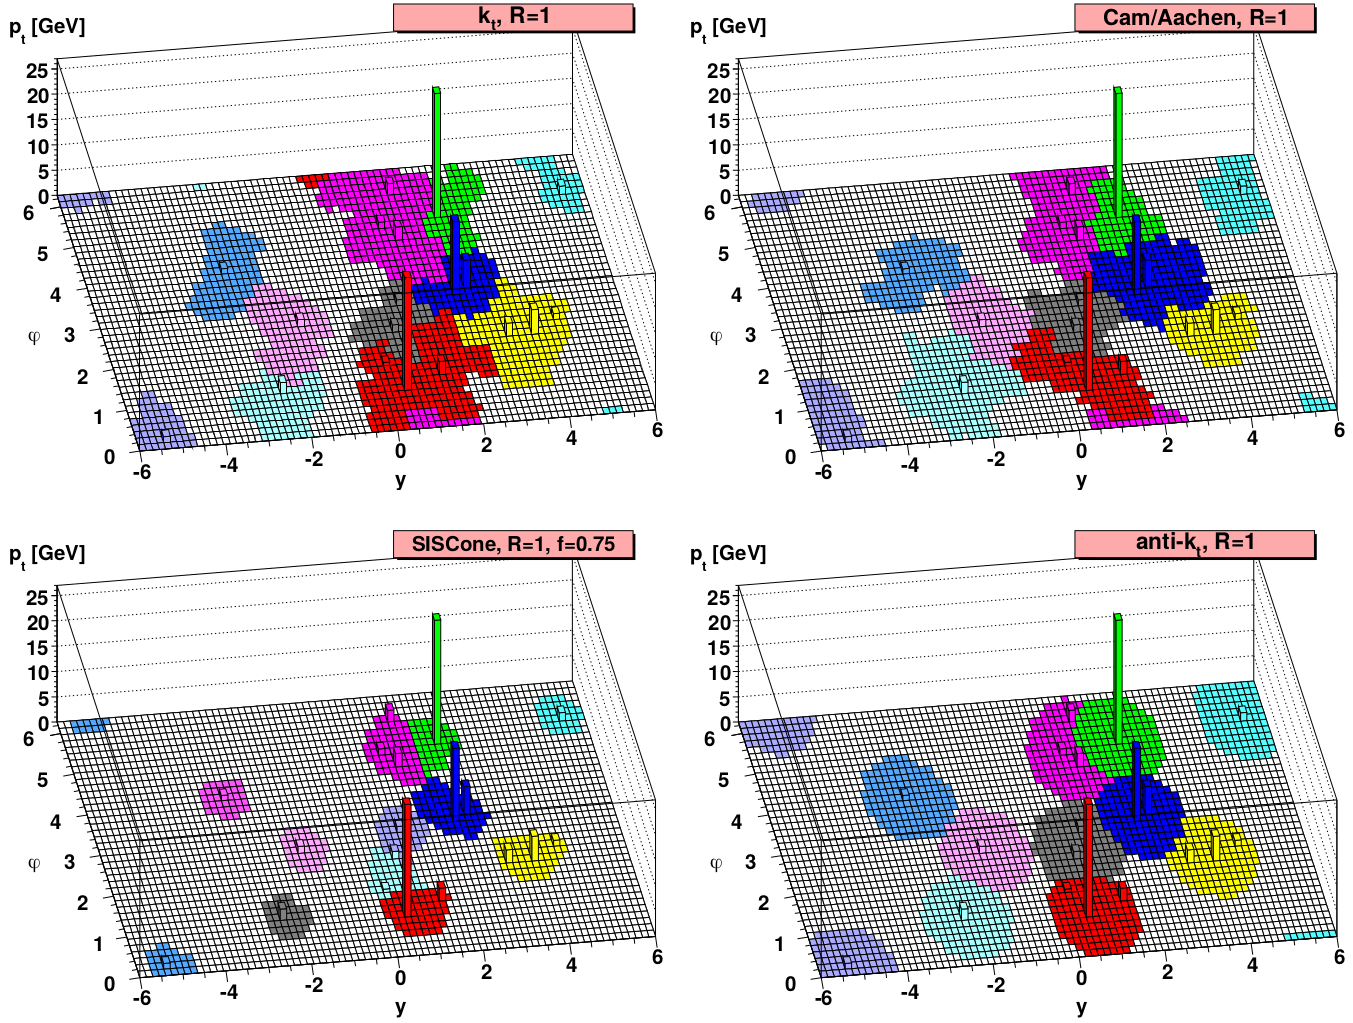
\includegraphics[width=.8\textwidth]{\PhDthesisdir/contents/chapter-JERC/reconstruction_des_jets/forme_des_jets.png}
\caption{Formes des jets reconstruits à partir de différents algorithmes pour un même événement~\cite{Cacciari_antikT}. En haut à gauche, \kT; en haut à droite, C/A; en bas à gauche, \textsc{SISCone}; en bas à droite, anti-\kT. L'algorithme anti-\kT\ permet d'obtenir des jets de forme régulière, conique.}
\label{fig-chapter-JERC-section-jets_reco-subsec-algo-examples}
\end{figure}
\par Le temps de calcul de ces algorithmes est un enjeu majeur au LHC.
Leurs temps d'exécution sont représentés en fonction du nombre d'événements d'empilement sur la figure~\ref{fig-chapter-JERC-section-jets_reco-subsec-algo-perfs}.
L'algorithme anti-\kT\ se place parmi les algorithmes les plus rapides.
Dans les conditions des collisions proton-proton du LHC, il permet le traitement d'un événement en moins d'une milliseconde.
C'est cet algorithme de regroupement qui est utilisé dans le cadre de l'expérience CMS.
\begin{figure}[h]
\centering
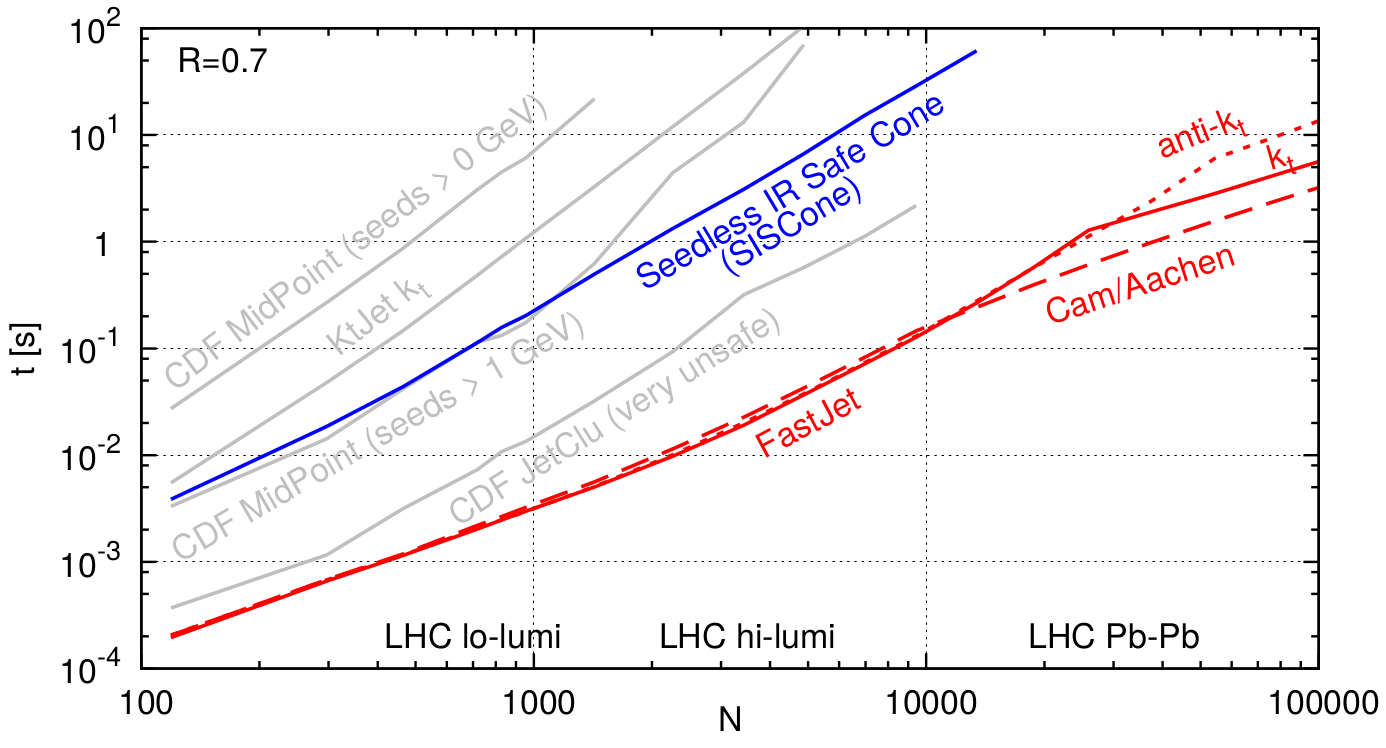
\includegraphics[width=.6\textwidth]{\PhDthesisdir/contents/chapter-JERC/reconstruction_des_jets/temps_de_calcul.png}
\caption{Temps de reconstruction d'un empilement d'un événement di-jets avec $N$ événements ne produisant que des jets de bas \pT\ pour différents algorithmes de reconstruction des jets.} % 50 GeV
\label{fig-chapter-JERC-section-jets_reco-subsec-algo-perfs}
\end{figure}
\subsection{Identification des jets dans CMS}\label{chapter-JERC-section-jets_reco-subsec-jetID}
Les jets ainsi reconstruits à l'aide des algorithmes de recombinaison sont en fait des \og candidats \fg{} jets.
À l'instar des particules individuelles, des critères d'identification leur sont appliqués afin de rejeter le bruit de fond et s'assurer de la qualité des jets ainsi reconstruits.
\par Ces critères reposent sur les caractéristiques des candidats jets comme la fraction d'énergie provenant de leurs constituants neutres ou encore le nombre de ces constituants.
Ces critères dépendent des années de prise de données et de la pseudo-rapidité du jet, \ie\ de la région du détecteur dans laquelle il se trouve.
\par Les critères utilisés pour les années 2016, 2017 et 2018, listés page~\pageref{tab-chapter-JERC-section-jets_reco-subsec-jetID-2017UL}, permettent d'obtenir une efficacité d'identification des jets supérieure à \SI{99}{\%} dans chacune des régions en $\eta$ du détecteur.
La réjection du bruit de fond est supérieure à \SI{98}{\%} pour $\abs{\eta}\leq\num{3.0}$ et supérieure à \SI{36}{\%} pour $\abs{\eta}>\num{3.0}$.
\begin{table}[p]
\centering
\begin{tabularx}{\textwidth}{lcYcY}
\toprule
Propriété du jet à identifier & $\abs{\eta}\leq\num{2.4}$ & $\num{2.4}<\abs{\eta}\leq\num{2.7}$ & $\num{2.7}<\abs{\eta}\leq\num{3.0}$ & $\num{3.0}<\abs{\eta}$ \\
\midrule
Fraction d'énergie\\
\labelitemi\ hadronique neutre & $<\num{0.90}$ & $<\num{0.90}$ & $<\num{0.98}$ & \\
\labelitemi\ électromagnétique neutre & $<\num{0.90}$ & $<\num{0.90}$ & $>\num{0.01}$ & $<\num{0.90}$ \\
\labelitemi\ hadronique chargée & $>\num{0}$ &&&\\
\labelitemi\ électromagnétique chargée & $<\num{0.99}$ &&&\\
\midrule
Nombre de constituants\\
\labelitemi\ neutres & $>\num{1}$ & $>\num{1}$ & $>\num{2}$ & $>\num{10}$ \\
\labelitemi\ chargés & $>\num{0}$ &&&\\
\bottomrule
\end{tabularx}

\caption{Critères d'identification des jets à CMS pour l'analyse des données de 2016.}
\label{tab-chapter-JERC-section-jets_reco-subsec-jetID-2016}
\end{table}
\begin{table}[p]
\centering
\begin{tabularx}{\textwidth}{lcYcY}
\toprule
Propriété du jet à identifier & $\abs{\eta}\leq\num{2.4}$ & $\num{2.4}<\abs{\eta}\leq\num{2.7}$ & $\num{2.7}<\abs{\eta}\leq\num{3.0}$ & $\num{3.0}<\abs{\eta}$ \\
\midrule
Fraction d'énergie\\
\labelitemi\ hadronique neutre & $<\num{0.90}$ & $<\num{0.90}$ &  & $>\num{0.02}$ \\
\labelitemi\ électromagnétique neutre & $<\num{0.90}$ & $<\num{0.90}$ & $<\num{0.99}$ et $>\num{0.02}$ & $<\num{0.90}$ \\
\labelitemi\ hadronique chargée & $>\num{0}$ &&&\\
\labelitemi\ électromagnétique chargée & $<\num{0.8}$ \\
\labelitemi\ muonique & $<\num{0.8}$ & $<\num{0.8}$ \\
\midrule
Nombre de constituants & $>\num{1}$ & $>\num{1}$\\
\labelitemi\ neutres & & & $>\num{2}$ & $>\num{10}$ \\
\labelitemi\ chargés & $>\num{0}$ &&&\\
\bottomrule
\end{tabularx}

\caption{Critères d'identification des jets à CMS pour l'analyse des données de 2017.}
\label{tab-chapter-JERC-section-jets_reco-subsec-jetID-2017}
\end{table}
\begin{table}[p]
\centering
\begin{tabularx}{\textwidth}{lcYcY}
\toprule
Propriété du jet à identifier & $\abs{\eta}\leq\num{2.6}$ & $\num{2.6}<\abs{\eta}\leq\num{2.7}$ & $\num{2.7}<\abs{\eta}\leq\num{3.0}$ & $\num{3.0}<\abs{\eta}\leq\num{5.0}$ \\
\midrule
Fraction d'énergie\\
\labelitemi\ hadronique neutre & $<\num{0.90}$ & $<\num{0.90}$ &  & $>\num{0.2}$ \\
\labelitemi\ électromagnétique neutre & $<\num{0.90}$ & $<\num{0.99}$ & $<\num{0.99}$ et $>\num{0.02}$ & $<\num{0.90}$ \\
\labelitemi\ hadronique chargée & $>\num{0}$ &&&\\
\midrule
Nombre de constituants & $>\num{1}$\\
\labelitemi\ neutres & & & $>\num{2}$ & $>\num{10}$ \\
\labelitemi\ chargés & $>\num{0}$ & $>\num{0}$ &&\\
\bottomrule
\end{tabularx}

\caption{Critères d'identification des jets à CMS pour l'analyse des données de 2018.}
\label{tab-chapter-JERC-section-jets_reco-subsec-jetID-2018}
\end{table}
\begin{table}[p]
\centering
\begin{tabularx}{\textwidth}{lcYcY}
\toprule
Propriété du jet à identifier & $\abs{\eta}\leq\num{2.6}$ & $\num{2.6}<\abs{\eta}\leq\num{2.7}$ & $\num{2.7}<\abs{\eta}\leq\num{3.0}$ & $\num{3.0}<\abs{\eta}\leq\num{5.0}$ \\
\midrule
Fraction d'énergie\\
\labelitemi\ hadronique neutre & $<\num{0.90}$ & $<\num{0.90}$ &  & $>\num{0.2}$ \\
\labelitemi\ électromagnétique neutre & $<\num{0.90}$ & $<\num{0.99}$ & $<\num{0.99}$ et $>\num{0.01}$ & $<\num{0.90}$ \\
\labelitemi\ hadronique chargée & $>\num{0}$ &&&\\
\labelitemi\ électromagnétique chargée & $<\num{0.8}$ & $<\num{0.8}$ \\
\labelitemi\ muonique & $<\num{0.8}$ & $<\num{0.8}$ \\
\midrule
Nombre de constituants & $>\num{1}$\\
\labelitemi\ neutres & & & $>\num{1}$ & $>\num{10}$ \\
\labelitemi\ chargés & $>\num{0}$ & $>\num{0}$ &&\\
\bottomrule
\end{tabularx}

\caption{Critères d'identification des jets à CMS pour l'analyse des données de 2017-UL.}
\label{tab-chapter-JERC-section-jets_reco-subsec-jetID-2017UL}
\end{table}
\subsection{Saveur des jets}\label{chapter-JERC-section-jets_reco-subsec-flavor}
b-tagging

\begin{figure}
\centering
\begin{tikzpicture}[scale=1.5]
\def\trackerrin{.100}
\def\trackerrout{1.185}
\def\trackercolor{ltcolorgray1}

\def\ECALrin{1.290}
\def\ECALrout{1.811}
\def\ECALcolor{ltcolorgreen1}

\def\HCALrin{1.812}
\def\HCALrout{2.854}
\def\HCALcolor{ltcoloryellow3}

\def\Solenrin{2.950}
\def\Solenrout{3.800}
\def\Solencolor{ltcolorgray2}

\def\ironryrina{3.850}
\def\ironryrouta{4.000}
\def\muonrina{4.020}
\def\muonrouta{4.400}
\def\ironryrinb{4.420}
\def\ironryroutb{4.880}
\def\muonrinb{4.905}
\def\muonroutb{5.285}
\def\ironryrinc{5.300}
\def\ironryroutc{5.960}
\def\muonrinc{5.975}
\def\muonroutc{6.355}
\def\ironryrind{6.375}
\def\ironryroutd{6.980}
\def\muonrind{7.000}
\def\muonroutd{7.380}
\def\muoncolor{ltcoloryellow1}
\def\ironrycolor{ltcolorred2}

\def\printele#1{
\draw [thick, ltcolorred] (0,0) arc (#1-90:#1-90+27:3) coordinate (eledeposit);
\draw [ltcolorred] (#1-5:1.25) node {\ele};
}
\def\printmu#1{
\draw [thick, ltcolorblue] (0,0) arc (#1-90:#1-90+33:6) arc (#1-90+33:#1-90:-12) node{\mu};
\draw [ltcolorblue] (#1-7:1.5) node {\mu};
}

\def\printantiele#1{
\draw [thick, ltcolorred] (0,0) arc (#1-90:#1-90-27:-3) coordinate (eledeposit);
\draw [ltcolorred] (#1-7:1.5) node {\ele};
%\draw [ltcolorred4, ultra thick] (eledeposit)--+(#1+25:\ECALrout);
}
\def\printantimu#1{
\draw [thick, ltcolorblue] (0,0) arc (#1-90:#1-90-33:-6) arc (#1-90-33:#1-90:12);
\draw [ltcolorblue] (#1-7:1.5) node {\mu};
}

\def\printtauh#1{
\draw [thick, ltcolorgreen4] (0,0) arc (#1-90:#1-90+11:10) ;
\draw [thick, ltcolorgreen4] (0,0) arc (#1-90:#1-90+6:20) ;
\draw [thick, ltcolorgreen4] (0,0) arc (#1-90:#1-90-11:-10) ;
\draw [ltcolorgreen4] (#1-12:1.5) node {\tauh};
}
\def\printantitauh#1{
\draw [thick, ltcolorgreen4] (0,0) arc (#1-90:#1-90-11:-10) ;
\draw [thick, ltcolorgreen4] (0,0) arc (#1-90:#1-90-6:-20) ;
\draw [thick, ltcolorgreen4] (0,0) arc (#1-90:#1-90+11:10) ;
\draw [ltcolorgreen4] (#1-12:1.5) node {\tauh};
}

\def\printjetnolabel#1{
\draw [thick, ltcolororange] (0,0) arc (#1-90+10:#1-90+22+10:5) ;
\draw [thick, ltcolororange] (0,0) arc (#1-90+5:#1-90+12+5:10) ;
\draw [thick, ltcolororange] (0,0) arc (#1-90:#1-90-22:-5) ;
\draw [thick, ltcolororange] (0,0) arc (#1-90:#1-90+6:20) ;
\draw [thick, ltcolororange] (0,0) arc (#1-90+5:#1-90+8+5:10) ;
\draw [thick, ltcolororange] (0,0) arc (#1-90:#1-90-11:-10) ;
\draw [thick, ltcolororange] (0,0) arc (#1-90:#1-90+11:10) ;
}

\def\printjet#1{
\printjetnolabel{#1}
\draw [ltcolororange] (#1-25:.5) node {jet};
}

\def\printjetfake#1{
\printjet{#1}
\draw [thick, ltcolorgreen4] (0,0) arc (#1-90:#1-90+11:10) ;
\draw [thick, ltcolorgreen4] (0,0) arc (#1-90:#1-90+6:20) ;
\draw [thick, ltcolorgreen4] (0,0) arc (#1-90:#1-90-11:-10) ;
\draw [ltcolorgreen4] (#1-17:1.5) node {f.\tauh};
}

\def\printdeposit#1#2#3#4{
\fill [#1] (#2-2:#3) arc (#2-2:#2+2:#3) -- (#2+2:#4) arc (#2+2:#2-2:#4) ;
}

\def\printECALdeposit#1#2{\printdeposit{#1}{#2}{\ECALrin}{\ECALrout}}
\def\printHCALdeposit#1#2{\printdeposit{#1}{#2}{\HCALrin}{\HCALrout}}

\def\printtauhdeposit#1{
\printHCALdeposit{ltcoloryellow4}{#1+3}
\printHCALdeposit{ltcoloryellow4}{#1+5}
\printHCALdeposit{ltcoloryellow4}{#1-5}
}

\def\printjetdeposit#1{
\printHCALdeposit{ltcoloryellow4}{#1+3}
\printHCALdeposit{ltcoloryellow4}{#1+5}
\printHCALdeposit{ltcoloryellow4}{#1-5}
\printHCALdeposit{ltcoloryellow4}{#1+21}
\printHCALdeposit{ltcoloryellow4}{#1+11}
\printHCALdeposit{ltcoloryellow4}{#1-11}
}

\def\printMuChSigA#1#2{
\fill [red] (#1-7.5+20*#2:\muonrina) arc (#1-7.5+20*#2:#1+7.5+20*#2:\muonrina) -- (#1+7.5+20*#2:\muonrouta) arc (#1+7.5+20*#2:#1-7.5+20*#2:\muonrouta) ;
}
\def\printMuChSigB#1#2{
\fill [red] (#1-7.5+20*#2:\muonrinb) arc (#1-7.5+20*#2:#1+7.5+20*#2:\muonrinb) -- (#1+7.5+20*#2:\muonroutb) arc (#1+7.5+20*#2:#1-7.5+20*#2:\muonroutb) ;
}
\def\printMuChSigC#1#2{
\fill [red] (#1-7.5+20*#2:\muonrinc) arc (#1-7.5+20*#2:#1+7.5+20*#2:\muonrinc) -- (#1+7.5+20*#2:\muonroutc) arc (#1+7.5+20*#2:#1-7.5+20*#2:\muonroutc) ;
}
\def\printMuChSigD#1#2{
\fill [red] (#1-7.5+20*#2:\muonrind) arc (#1-7.5+20*#2:#1+7.5+20*#2:\muonrind) -- (#1+7.5+20*#2:\muonroutd) arc (#1+7.5+20*#2:#1-7.5+20*#2:\muonroutd) ;
}

\foreach\jetangle in {120,-145}{
\printbigjetnolabel{\jetangle}
\draw (\jetangle:2.5) node {jet} ;
}

\def\Bjetangle{30}
\def\Bhaddronangle{5}
\def\Bhaddronflight{.75}

\def\CurrentVertex{(\Bhaddronangle:\Bhaddronflight)}

\draw [thick, dotted] (0,0) -- \CurrentVertex ;

{
\def\jetcolor{ltcolorred}
\printjetnolabel{\Bjetangle}
\draw [\jetcolor] (\Bjetangle:2)+(1.5,.75) node {traces déplacées};
}
\begin{scope}
\clip circle (\Solenrin);
\printantimuonnolabel{\Bjetangle}
\end{scope}

\draw [\muoncolor] (\Bjetangle:4) +(0,{-2*\baselineskip}) node {lepton chargé};

\draw (\Bjetangle:4) + (-.125,-.5) circle (1.125);
\draw [-latex] (\Bjetangle:4) + (-.125,-1.625) --+ (-.125,-2) node [below] {jet de saveur lourde};

\draw (0,0) node [left] {PV} ;
\draw \CurrentVertex node [below right] {SV} ;

\fill (0,0) circle (2pt);
\fill \CurrentVertex circle (2pt);

\draw [dashed] \CurrentVertex --+ (\Bjetangle:-.8);

\draw [red, latex-latex] (0,0)--+ (-90+\Bjetangle:{\Bhaddronflight*sin(\Bjetangle-\Bhaddronangle)}) node [below right] {IP};
\end{tikzpicture}
\end{figure}
\subsection{Énergie transverse manquante}\label{chapter-LHC-section-evt_reco-subsec-MET}

\subsection{Taus hadroniques}\label{chapter-HTT_analysis-section-objects-taus}

\begin{wrapfigure}{R}{.4\textwidth}
\centering
\begin{fmffile}{tau_to_tauh-3prongs}%\fmfstraight
\begin{fmfchar*}(30,20)
  \fmfleft{taui}
  \fmfright{l1,l2,l3,f1,f2,f3,nuout}
  \fmf{fermion, label=$\leptau$, l.side=left, tension=2}{taui,v1}
  \fmf{fermion}{v1,nuout}
  \fmf{phantom}{v1,l1}
  \fmffreeze
  \fmflabel{$\nutau$}{nuout}
  \fmf{boson, label=$\Wbosonminus$, l.side=right, tension=2}{v1,v2}
  \fmf{phantom}{v2,td1,l1}
  \fmf{phantom}{v2,td2,l2}
  \fmf{phantom}{v2,td3,l3}
  \fmffreeze
  \fmf{plain}{td3,v2,td1}
  \fmfblob{.15w}{td2}
  \fmf{plain}{td2,l1}
  \fmf{plain}{td2,l2}
  \fmf{plain}{td2,l3}
  \fmflabel{$\hadron^-$}{l1}
  \fmflabel{$\hadron^-$}{l2}
  \fmflabel{$\hadron^+$}{l3}
  \fmfdot{v1,v2}
\end{fmfchar*}
\end{fmffile}

\vspace{\baselineskip}
\caption{Diagramme de Feynman de désintégration hadronique d'un \leptau.}
\label{fig-fgraph-tau_to_tauh}
\end{wrapfigure}
Lors d'une désintégration hadronique d'un lepton tau, une paire de quarks est émise.
Il s'en suit donc un processus d'hadronisation, phénomène à l'origine de la formation des jets, ce qui est exposé dans le chapitre~\refChJERC.
Du lepton tau résulte alors un ensemble de hadrons, comme illustré sur la figure~\ref{fig-fgraph-tau_to_tauh}.
Ces hadrons, en général trois ou moins, sont éventuellement accompagnés de particules neutres, principalement des \pionnull.
Ces derniers se désintégrant majoritairement en deux photons.
L'ensemble de ces particule forme un \og tau hadronique \fg, noté \tauh, et est initialement identifié comme un jet.
\subsubsection{Obtention de candidats tau hadronique}
L'identification des taus hadroniques est réalisée par l'algorithme \emph{Hadrons Plus Strips} (HPS)~\cite{Khachatryan:2015dfa,Sirunyan:2018pgf} à partir des jets reconstruits par l'algorithme de \PF\ vérifiant $\pT>\SI{14}{\GeV}$ et $\abs{\eta}<\num{2.5}$.
Les hadrons chargés contenus dans le jet initial tels que $\pT>\SI{0.5}{\GeV}$ et de paramètre d'impact transverse $d_{xy}<\SI{0.1}{\centi\meter}$ vis-à-vis du vertex primaire principal sont utilisés pour former des candidats \tauh.
\par
Afin d'identifier les dépôts d'énergie dans le ECAL dus aux \pionnull, les photons et les électrons contenus dans le jet initial sont regroupés en bandes (\emph{strips}).
La construction d'une bande est un procédé itératif:
\begin{enumerate}
\item Une bande est créée à partir de l'électron ou du photon ($\ele/\photon$) de plus haut \pT\ contenu dans le jet initial et n'ayant pas déjà été associé à une bande. La position de cette particule dans le plan $(\eta,\phi)$, ainsi que son \pT, sont associés à la bande.
\item L'électron ou photon de plus haut \pT\ restant est ajouté à la bande s'il est situé à une distance par rapport à la bande dans le plan $(\eta,\phi)$ telle que
\begin{align}
\Delta\eta < f\left(\pT^{(\ele/\photon)}\right) + f\left(\pT^\text{bande}\right) \msep& f(\pT) = \num{0.20} (\pT [\SI{}{\GeV}])^{-\num{0.66}}\\
\Delta\phi < g\left(\pT^{(\ele/\photon)}\right) + g\left(\pT^\text{bande}\right) \msep& g(\pT) = \num{0.35} (\pT [\SI{}{\GeV}])^{-\num{0.71}}
\end{align}
avec $\pT^{(\ele/\photon)}$ l'impulsion transverse de l'électron ou du photon à ajouter à la bande et $\pT^\text{bande}$ l'impulsion transverse associée à la bande avant ajout de l'électron ou du photon.\\
Si l'ajout se fait, la bande est mise à jour selon
\begin{align}
\pT^\text{bande} &= \sum_{\ele/\photon\in\text{bande}}\pT^{(\ele/\photon)}\mend[,]\\
\eta^\text{bande} &= \frac{1}{\pT^\text{bande}} \sum_{\ele/\photon\in\text{bande}}\pT^{(\ele/\photon)} \eta_{(\ele/\photon)}\mend[,]\\
\phi^\text{bande} &= \frac{1}{\pT^\text{bande}} \sum_{\ele/\photon\in\text{bande}}\pT^{(\ele/\photon)} \phi_{(\ele/\photon)}\mend[,]
\end{align}
ce qui rend la bande dynamique lors de sa construction.
Les dimensions de la bande sont limitées à $\num{0.05}<\Delta\eta<\num{0.15}$ et $\num{0.05}<\Delta\phi<\num{0.3}$.
\item L'étape précédente est répétée jusqu'à ce qu'une limite de taille de la bande soit atteinte ou qu'il ne reste plus d'électron ni de photon tels que $\pT>\SI{0.5}{\GeV}$ dans la zone de la bande.
\item Les éléments associés à la bande sont retirés de la liste des électrons et photons en attente d'association à une bande.
\item Le procédé reprend à l'étape 1.
\end{enumerate}
Toute bande vérifiant $\pT>\SI{2.5}{\GeV}$ est considérée comme un candidat \pionnull.
\par
Des candidats \tauh\ compatibles avec un des modes de désintégration hadronique du tau sont ainsi formés à partir de toutes les combinaisons possibles de hadrons chargés et de candidats \pionnull.
\subsubsection{Modes de désintégration hadronique du tau}
Les modes de désintégration (\emph{Decay Modes}, DM) considérés dans l'analyse sont ainsi listé dans le tableau~\ref{tab-tauh-DMs}.
À chaque DM correspond une valeur afin de le désigner, définie comme
\begin{equation}
\text{DM} = 5\times(N_{\hadronpm}-1) - N_{\pionnull}
\end{equation}
où $N_{\hadronpm}$ est le nombre de hadrons chargés et $N_{\pionnull}$ le nombre de \pionnull\ contenus dans le \tauh.
Lorsqu'un des hadrons chargés n'est pas reconstruit, il est possible d'obtenir les DM 5, 6 ou 7.
Ces cas de figure sont largement contaminés par le bruit de fond \og QCD multijet \fg, ils sont donc rejetés dans l'analyse.
\begin{table}[h]
\centering
\begin{tabular}{clc}
\toprule
Code & Mode de désintégration & \BR{} (\SI{}{\%})\\
\midrule
0 & $\leptau\to \hadronminus \antinutau$ & \num{11.51} \\
1 & $\leptau\to \hadronminus \pionnull \antinutau$ & \num{25.93} \\
2 & $\leptau\to \hadronminus \pionnull\pionnull \antinutau$ & \num{9.48} \\
10 & $\leptau\to \hadronminus \hadronminus\hadronplus \antinutau$ & \num{9.80} \\
11 & $\leptau\to \hadronminus \hadronminus\hadronplus\pionnull\antinutau$ & \num{4.76} \\
\bottomrule
\end{tabular}
\caption[Modes de désintégration du \tau\ considérés.]{Modes de désintégration du \tau\ considérés. La désintégration d'un \leptau\ correspondant au DM, ainsi que le rapport de branchement $\leptau\to\tauh^-$ correspondant~\cite{PDG_booklet_2020} sont également donnés.}
\label{tab-tauh-DMs}
\end{table}
\par
Certains DM présentent des contraintes supplémentaires sur la masse du \tauh:
\begin{align*}
\text{DM 1:} && \SI{0.3}{\GeV} < m_{\tauh} < \num{1.3}\sqrt{\frac{\pT[\SI{}{\GeV}]}{100}} \SI{}{\GeV}\mend[,]\\
\text{DM 2:} && \SI{0.4}{\GeV} < m_{\tauh} < \num{1.2}\sqrt{\frac{\pT[\SI{}{\GeV}]}{100}} \SI{}{\GeV}\mend[,]\\
\text{DM 10 et 11:} && \SI{0.8}{\GeV} < m_{\tauh} < \SI{1.5}{\GeV}\mend[,]\\
\end{align*}
et, dans le cas du DM 10, les traces des hadrons chargés doivent provenir du même vertex dans la limite de $\Delta z < \SI{0.4}{\centi\meter}$.
\subsubsection{Sélection d'un candidat \tauh}
Il est possible d'obtenir plusieurs candidats \tauh\ au sein d'un même jet.
Des critères de qualité sur les candidats leur sont alors imposés.
\par
Par conservation, la somme des charges électriques des hadrons contenus dans le candidat \tauh\ doit valoir $\pm1$.
Ces hadrons chargés doivent de plus être contenus dans le cône dit \og de signal \fg{} défini et contraint selon
\begin{equation}
\Delta R_\text{sig} = \frac{\SI{3}{\GeV}}{\pT^{(\tauh)}}
\msep
\num{0.05} < \Delta R_\text{sig} < \num{0.1}
\mend
\end{equation}
Les centres des bandes du candidat \tauh\ doivent également se situer dans ce cône.
S'il reste plusieurs candidats à ce stade, celui de plus haut \pT\ est retenu.
Il existe donc au plus un \tauh\ par jet.
\subsubsection{Mauvaises reconstruction de \tauh}
Un \tauh\ peut être reconstruit à partir de jets n'étant pas des \tauh, d'électrons ou de muons.
Afin de réduire la quantité de mauvais \tauh\ (\ftauh), un réseau de neurones profond convolutionnel (DNN)~\cite{DNN} a été développé à CMS.
Il s'agit de l'algorithme \DEEPTAU~\cite{CMS-DP-2019-033} qui fournit les discriminateurs
\texttt{deepTau vs jet},
\texttt{deepTau anti-electron} et
\texttt{deepTau anti-muon}
utilisés dans cette analyse.
\par
Les points de fonctionnement utilisés pour chacun de ces discriminateurs dépendent de l'état final, comme présenté dans la section~\ref{chapter-HTT_analysis-section-selection}.
Les efficacités d'identification de chacun des points de fonctionnement existants sont donnés dans le tableau~\ref{tab-HTT_analysis-section-objects-taus-DEEPTAU_eff}.
Les taux d'identification de jet, électron ou muon comme étant un \tauh, \ie\ les faux positifs, dépendent de la nature des événements sur lesquels ces discriminateurs sont appliqués et se situent entre \num{e-4} et \num{e-2}.
\begin{table}[h]
\centering
\begin{tabular}{lcccccccc}
\toprule
Discriminateur & \emph{VVTight} & \emph{VTight} & \emph{Tight} & \emph{Medium} & \emph{Loose} & \emph{VLoose} & \emph{VVLoose} & \emph{VVVLoose}\\
\midrule
\texttt{vs jet} & \num{40} & \num{50} & \num{60} & \num{70} & \num{80} & \num{90} & \num{95} & \num{98} \\
\texttt{anti-electron} & \num{60} & \num{70} & \num{80} & \num{90} & \num{95} & \num{98} & \num{99} & \num{99.5} \\
\texttt{anti-muon} & - & - & \num{99.5} & \num{99.8} & \num{99.9} & \num{99.95} & - & - \\
\bottomrule
\end{tabular}
\caption[Efficacités d'identification de l'algorithme \DEEPTAU.]{Efficacités d'identification en \SI{}{\%} de l'algorithme \DEEPTAU\ pour chacun des points de fonctionnement disponibles~\cite{CMS-DP-2019-033,Androsov_deeptau}.}
\label{tab-HTT_analysis-section-objects-taus-DEEPTAU_eff}
\end{table}